\documentclass{article}
\usepackage{tikz}
\usetikzlibrary{arrows.meta, positioning, external}
\tikzexternalize

\title{TikZ Externalization Example}
\author{maketex}

\begin{document}
\maketitle

\texttt{maketex} handles TikZ externalization automatically, keeping cached
figure PDFs inside \texttt{.maketex/} instead of cluttering the project root.

\begin{figure}[h]
\centering
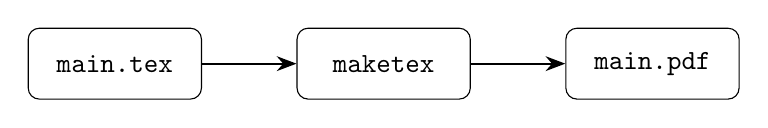
\begin{tikzpicture}[
  box/.style={draw, rounded corners, minimum width=2.2cm, minimum height=0.9cm, align=center},
  arrow/.style={-{Stealth[length=2.5mm]}, thick}
]
  \node[box] (tex) {\texttt{main.tex}};
  \node[box, right=1.2cm of tex] (mk) {\texttt{maketex}};
  \node[box, right=1.2cm of mk] (pdf) {\texttt{main.pdf}};
  \draw[arrow] (tex) -- (mk);
  \draw[arrow] (mk) -- (pdf);
\end{tikzpicture}
\caption{Build pipeline rendered with externalized TikZ.}
\end{figure}

\end{document}
